\documentclass[aspectratio=169]{beamer}
\usepackage{will_handley_beamer}
\usepackage{title_page}
\usepackage[normalem]{ulem}

% Commands
% --------
% - \arxiv{arxiv number}
% - \arxiv{<number>}            arxiv.org/abs/<number>
% - \oldarxiv{<arxiv number>}   arxiv.org/<number>
% - \doi{<doi>}                 doi.org/<doi>
% - \xkcd{<number>}             xkcd.com/<number>
% - \email{<email>}             <<email>>
% - \tthref{<website>}          <website>
% - \av[dist]{<quantity>}       <quantity>_{dist}
% - \student{<name>}{<detail>}{<photo>}

% Talk details
% ------------
\title{Next-Generation Model Comparison for Primordial Cosmology}
\date{21\textsuperscript{st} January 2025}

\begin{document}

\begin{frame}
    \titlepage
\end{frame}

\begin{frame}
    \frametitle{Bayesian Inference Challenges in 21cm Cosmology}
    \begin{columns}[T]
        \column{0.49\textwidth}
        \begin{block}{Computational Challenges}
            \begin{itemize}
                \item High-dimensional parameter spaces (20-100+ parameters)
                \item Complex, multimodal posteriors
                \item Expensive likelihood evaluations
                \item Months of computation time
                \item Model comparison bottlenecks
            \end{itemize}
        \end{block}
        \column{0.49\textwidth}
        \begin{block}{Physical Challenges}
            \begin{itemize}
                \item Foreground contamination 10$^5$× stronger than signal
                \item Instrumental systematics
                \item Ionospheric effects
                \item Degeneracies between astrophysics and cosmology
                \item Need for robust uncertainty quantification
            \end{itemize}
        \end{block}
    \end{columns}
    \vspace{10pt}
    \begin{center}
        \Large
        \textbf{These challenges demand new computational approaches}
    \end{center}
\end{frame}

\begin{frame}
    \frametitle{GPU Computing: Beyond Machine Learning}
    \begin{columns}
        \column{0.48\textwidth}
        \begin{block}{GPU vs CPU for Scientific Computing}
            \begin{itemize}
                \item \textbf{CPU}: Few powerful cores (10s), complex control.
                \item \textbf{GPU}: Many simple cores (1000s), simple control.
                \item \textbf{Memory bandwidth}: GPU ~10× faster than CPU.
                \item \textbf{Perfect for}: Independent parallel tasks.
                \item \textbf{Scientific algorithms}: MCMC chains, likelihood evaluations, simulations.
            \end{itemize}
        \end{block}
        \column{0.48\textwidth}
        \begin{block}{HPC Landscape Evolution}
            \begin{itemize}
                \item HPC transitioning to GPU-based architectures.
                \item ML adoption accelerating hardware development.
                \item Legacy CPU codes require modernization.
            \end{itemize}
        \end{block}
        \begin{block}{Key Point}
            \begin{center}
                \textbf{GPU $\neq$ Machine Learning}\\
                GPUs accelerate any parallel algorithm
            \end{center}
        \end{block}
    \end{columns}
\end{frame}

\begin{frame}
    \frametitle{Modern Languages: Two Independent Capabilities}
    \begin{center}
        \textbf{Differentiable programming languages}: JAX, PyTorch, TensorFlow, Julia, Stan, \ldots
    \end{center}
    \vspace{-5pt}
    \begin{columns}
        \column{0.48\textwidth}
        \begin{block}{Capability 1: Free Gradients}
            \begin{itemize}
                \item \textbf{Automatic differentiation}: $\nabla_\theta \log \mathcal{L}(\theta)$.
                \item Enables gradient-based MCMC (HMC, NUTS).
                \item Essential for modern optimization.
            \end{itemize}
        \end{block}
        \begin{block}{Traditional Physics Benefits}
            \begin{itemize}
                \item \textbf{Nested sampling}: Massive parallelization.
                \item \textbf{21cm signals}: Vectorized across frequency/time/angle.
                \item \textbf{N-body sims}: GPU acceleration.
            \end{itemize}
        \end{block}
        \column{0.48\textwidth}
        \begin{block}{Capability 2: GPU Parallelization}
            \begin{itemize}
                \item \textbf{Vectorization across ensembles}.
                \item Run 1000s of parallel chains/particles.
                \item Evaluate likelihoods simultaneously.
            \end{itemize}
        \end{block}
        \begin{block}{Key Insight: Often Confused}
            \begin{center}
                \textbf{These are completely independent.}\\
                \textbf{People mistake one for the other.}\\
                You can use gradients on CPU.\\
                You can GPU parallelize without gradients.\\
                \textbf{They serve different purposes.}
            \end{center}
        \end{block}
    \end{columns}
\end{frame}

\begin{frame}
    \frametitle{BlackJAX: GPU Native Sampling}
    \framesubtitle<1-10>{Gradient descent: inference at speed}
    \framesubtitle<11-19>{Metropolis-Hastings: error bars}
    \framesubtitle<20-28>{emcee: adaptive ensemble algorithms}
    \framesubtitle<29-36>{Nested sampling: model comparison}
    \framesubtitle<37-44>{Hamiltonian Monte Carlo: inference with gradients}
    \student{david_yallup}{David Yallup}{Postdoc}
    \begin{columns}
        \column{0.48\textwidth}
        \vspace{-10pt}
        \begin{itemize}
            \item Sampling traditionally CPU-bound.
            \item Different algorithms, same GPU challenge.
            \item Need unified GPU-native framework.
            \item From optimization to model comparison.
        \end{itemize}
        \vspace{10pt}
        \begin{itemize}
            \item BlackJAX: Full JAX ecosystem.
            \item All algorithms GPU-accelerated.
            \item Gradient descent through nested sampling.
            \item Unified interface, maximum performance.
        \end{itemize}
        \vspace{5pt}
        \begin{itemize}
            \item Framework: more like \texttt{numpy} or \texttt{scipy} than \texttt{cobaya} or \texttt{cosmosis}.
        \end{itemize}
        \column{0.48\textwidth}
        \vspace{10pt}
        \includegraphics<1>[width=\textwidth,page=1]{figures/himmelblau_gradient_ascent}%
        \includegraphics<2>[width=\textwidth,page=2]{figures/himmelblau_gradient_ascent}%
        \includegraphics<3>[width=\textwidth,page=3]{figures/himmelblau_gradient_ascent}%
        \includegraphics<4>[width=\textwidth,page=4]{figures/himmelblau_gradient_ascent}%
        \includegraphics<5>[width=\textwidth,page=5]{figures/himmelblau_gradient_ascent}%
        \includegraphics<6>[width=\textwidth,page=6]{figures/himmelblau_gradient_ascent}%
        \includegraphics<7>[width=\textwidth,page=7]{figures/himmelblau_gradient_ascent}%
        \includegraphics<8>[width=\textwidth,page=8]{figures/himmelblau_gradient_ascent}%
        \includegraphics<9>[width=\textwidth,page=9]{figures/himmelblau_gradient_ascent}%
        \includegraphics<10>[width=\textwidth,page=10]{figures/himmelblau_gradient_ascent}%
        \includegraphics<11>[width=\textwidth,page=1]{figures/himmelblau_mcmc}%
        \includegraphics<12>[width=\textwidth,page=2]{figures/himmelblau_mcmc}%
        \includegraphics<13>[width=\textwidth,page=3]{figures/himmelblau_mcmc}%
        \includegraphics<14>[width=\textwidth,page=4]{figures/himmelblau_mcmc}%
        \includegraphics<15>[width=\textwidth,page=5]{figures/himmelblau_mcmc}%
        \includegraphics<16>[width=\textwidth,page=6]{figures/himmelblau_mcmc}%
        \includegraphics<17>[width=\textwidth,page=7]{figures/himmelblau_mcmc}%
        \includegraphics<18>[width=\textwidth,page=8]{figures/himmelblau_mcmc}%
        \includegraphics<19>[width=\textwidth,page=9]{figures/himmelblau_mcmc}%
        \includegraphics<20>[width=\textwidth,page=1]{figures/himmelblau_emcee}%
        \includegraphics<21>[width=\textwidth,page=2]{figures/himmelblau_emcee}%
        \includegraphics<22>[width=\textwidth,page=3]{figures/himmelblau_emcee}%
        \includegraphics<23>[width=\textwidth,page=4]{figures/himmelblau_emcee}%
        \includegraphics<24>[width=\textwidth,page=5]{figures/himmelblau_emcee}%
        \includegraphics<25>[width=\textwidth,page=6]{figures/himmelblau_emcee}%
        \includegraphics<26>[width=\textwidth,page=7]{figures/himmelblau_emcee}%
        \includegraphics<27>[width=\textwidth,page=8]{figures/himmelblau_emcee}%
        \includegraphics<28>[width=\textwidth,page=9]{figures/himmelblau_emcee}%
        \includegraphics<29>[width=\textwidth,page=1]{figures/himmelblau_ns}%
        \includegraphics<30>[width=\textwidth,page=2]{figures/himmelblau_ns}%
        \includegraphics<31>[width=\textwidth,page=3]{figures/himmelblau_ns}%
        \includegraphics<32>[width=\textwidth,page=4]{figures/himmelblau_ns}%
        \includegraphics<33>[width=\textwidth,page=5]{figures/himmelblau_ns}%
        \includegraphics<34>[width=\textwidth,page=6]{figures/himmelblau_ns}%
        \includegraphics<35>[width=\textwidth,page=7]{figures/himmelblau_ns}%
        \includegraphics<36>[width=\textwidth,page=8]{figures/himmelblau_ns}%
        \includegraphics<37>[width=\textwidth,page=1]{figures/himmelblau_hmc}%
        \includegraphics<38>[width=\textwidth,page=2]{figures/himmelblau_hmc}%
        \includegraphics<39>[width=\textwidth,page=3]{figures/himmelblau_hmc}%
        \includegraphics<40>[width=\textwidth,page=4]{figures/himmelblau_hmc}%
        \includegraphics<41>[width=\textwidth,page=5]{figures/himmelblau_hmc}%
        \includegraphics<42>[width=\textwidth,page=6]{figures/himmelblau_hmc}%
        \includegraphics<43>[width=\textwidth,page=7]{figures/himmelblau_hmc}%
        \includegraphics<44>[width=\textwidth,page=8]{figures/himmelblau_hmc}%
    \end{columns}
\end{frame}

\begin{frame}
    \frametitle{Recent GPU-Accelerated Applications}
    \framesubtitle{Case study 1/4: CMB and Cosmic Shear \arxiv{2509.13307}}
    \student{toby_lovick}{Toby Lovick}{PhD}
    \begin{columns}
        \column{0.48\textwidth}
        \begin{itemize}
            \item \textbf{CMB (6 params)}: 300× speedup vs CPU PolyChord
            \item \textbf{Cosmic Shear (37 params)}: Days vs months
            \item \textbf{Method}: JAX neural emulators + GPU NS
            \item \textbf{Evidence}: Direct calculation with error bars
            \item \textbf{Models}: $\Lambda$CDM vs $w_0w_a$ comparison
            \item \textbf{Impact}: NS competitive with MCMC+evidence methods
        \end{itemize}
        \column{0.48\textwidth}
        \includegraphics<1>[width=\textwidth]{figures/cmbscaling.pdf}%
        \vspace{5pt}
        \includegraphics<2>[width=\textwidth]{figures/jaxSHEARfull.png}
        %\vspace{10pt}
        %\begin{block}{Key Insight: Classical > ML Gold Rush}
        %    \begin{itemize}
        %        \item \textbf{No machine learning}: Pure nested sampling
        %        \item \textbf{Statistical guarantees}: Proper uncertainties + evidence
        %        \item \textbf{Factor in training costs}: ML often slower end-to-end
        %        \item \textbf{Transparent algorithms}: No black boxes
        %    \end{itemize}
        %\end{block}
    \end{columns}
\end{frame}

\begin{frame}
    \frametitle{Recent GPU-Accelerated Applications}
    \framesubtitle{Case study 2/4: Bayesian Anomaly Detection for Type Ia Supernovae \arxiv{2509.13394}}
    \student{sam_leeney}{Sam Leeney}{PhD}
    \begin{columns}
        \column{0.48\textwidth}
        \begin{itemize}
            \item \textbf{Problem}: Manual photometric rejection not scalable for LSST
            \item \textbf{Solution}: Bayesian anomaly detection integrated into SALT3 fitting
            \item \textbf{Method}: Model contamination probability per measurement
            \item \textbf{Result}: Automatic outlier/corrupted band rejection
            \item \textbf{Finding}: Contaminants systematically brighter/bluer
            \item \textbf{Impact}: Essential for unbiased cosmology at scale
        \end{itemize}
        \column{0.48\textwidth}
        \vspace{10pt}
        \includegraphics<1>[width=\textwidth]{2509.13394/images/19ekb_light_curves_all_paper.png}%
        \includegraphics<2>[width=\textwidth]{2509.13394/images/recreated_contamination_plot.png}
    \end{columns}
\end{frame}

\begin{frame}
    \frametitle{Recent GPU-Accelerated Applications}
    \framesubtitle{Case study 3/4: Dark Energy vs Supernova Systematics \arxiv{2509.13220}}
    \student{adam_ormondroyd}{Adam Ormondroyd}{PhD}
    \begin{columns}
        \column{0.65\textwidth}
        \begin{itemize}
            \item \textbf{Question}: DESI+DES $w_0w_a$ preference - new physics or systematics?
            \item \textbf{Method}: Bayesian model comparison
            \item \textbf{Models}: Dynamic DE vs redshift-dependent SN bias
            \item \textbf{Result}: Systematics fit equally well with lower complexity
            \item \textbf{Evidence}: Favors systematic explanation
            \item \textbf{Lesson}: Test mundane before claiming exotic
        \end{itemize}
        \column{0.35\textwidth}
        \vspace{10pt}
        \includegraphics<1>[width=\textwidth]{2509.13220/plots/desidr2_des5yoffset_20_wa.pdf}%
        \includegraphics<2>[width=\textwidth]{2509.13220/plots/des5yoffset_20_wa.pdf}
    \end{columns}
\end{frame}

\begin{frame}
    \frametitle{Recent GPU-Accelerated Applications}
    \framesubtitle{Case study 4/4: Gravitational Wave Inference \arxiv{2509.04336}}
    \student{metha_prathaban}{Metha Prathaban}{PhD}
    \begin{columns}
        \column{0.48\textwidth}
        \begin{itemize}
            \item \textbf{Goal}: GPU-accelerate bilby's acceptance-walk NS
            \item \textbf{Implementation}: Faithful port to blackjax-ns
            \item \textbf{Performance}: 20-40× speedup for BBH
            \item \textbf{Validation}: Identical posteriors/evidences
            \item \textbf{Hardware}: Single GPU vs CPU clusters
            \item \textbf{Impact}: Clean baseline for future methods
        \end{itemize}
        \column{0.48\textwidth}
        \includegraphics<1>[width=\textwidth]{prathaban_handley_2509.04336/figures/8s_corner_comparison.pdf}%
        \includegraphics<2>[width=\textwidth]{prathaban_handley_2509.04336/figures/walltime_speedup.pdf}
    \end{columns}
\end{frame}

\begin{frame}
    \frametitle{The Future: AI in Scientific Code Development}
    \student{claude}{Claude Code}{AI Assistant}
    \vspace{-1em}
    \begin{columns}[T]
        \column{0.49\textwidth}
        \begin{block}{The Real AI Revolution: LLMs}
            The biggest impact of AI will not be in analyzing data, but in helping us write the code to do it.
            \begin{itemize}
                \item \textbf{Automated code translation}: LLMs can help port legacy Fortran/C++ models to modern, GPU-friendly \& differentiable frameworks like JAX or PyTorch.
            \end{itemize}
        \end{block}
        \column{0.49\textwidth}
        \begin{block}{The 80/20 Rule of Scientific Work}
            \begin{itemize}
                \item \textbf{80\% ``boring'' tasks}: Writing code, debugging, drafting \& reviewing papers, munging data, organising meetings...
                \item \textbf{20\% ``hard thinking''}: The actual scientific insight.
            \end{itemize}
            AI's biggest immediate impact is automating and accelerating the 80\%, freeing up human time for the 20\%.
        \end{block}
    \end{columns}
    \begin{alertblock}{Key Message}
        AI is not just a tool for analysis; it's about to fundamentally change how we develop, optimize, and deploy our science
    \end{alertblock}
\end{frame}


\begin{frame}
    \frametitle{Conclusions}
    \framesubtitle{\tthref{github.com/handley-lab/group}}
        \begin{enumerate}
            \item \textbf{GPU $\neq$ Machine Learning: Two Independent Capabilities}
                \begin{itemize}
                    \item GPUs accelerate any parallel algorithm.
                    \item Automatic differentiation + massive parallelization.
                    \item Often confused, serve different purposes.
                \end{itemize}
            \item \textbf{Classical Algorithms on GPU Competitive with ML State of the Art}
                \begin{itemize}
                    \item Traditional physics methods + GPU = superior performance.
                \end{itemize}
            \item \textbf{AI Accelerates Development as well as Computation}
                \begin{itemize}
                    \item LLMs solve the GPU porting challenge at scale.
                    \item 10× development speedup enables widespread adoption.
                \end{itemize}
        \end{enumerate}
        \vfill
        \begin{alertblock}{Get Started with GPU-Accelerated Sampling}
            \centering
            \Large
            \tthref{handley-lab.co.uk/nested-sampling-book}
        \end{alertblock}
    \tikz[overlay,remember picture]
        \node[anchor=north east] (A) at ($(current page.north east)+(0,0)$) {
        
\includegraphics[width=0.06\textheight]{people/adam_ormondroyd.jpg}%
        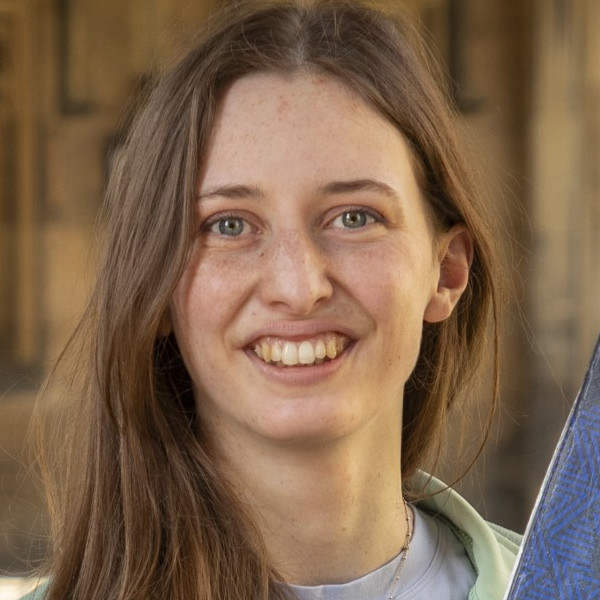
\includegraphics[width=0.06\textheight]{people/charlotte_priestley.jpg}%
        
\includegraphics[width=0.06\textheight]{people/claude.jpg}%
        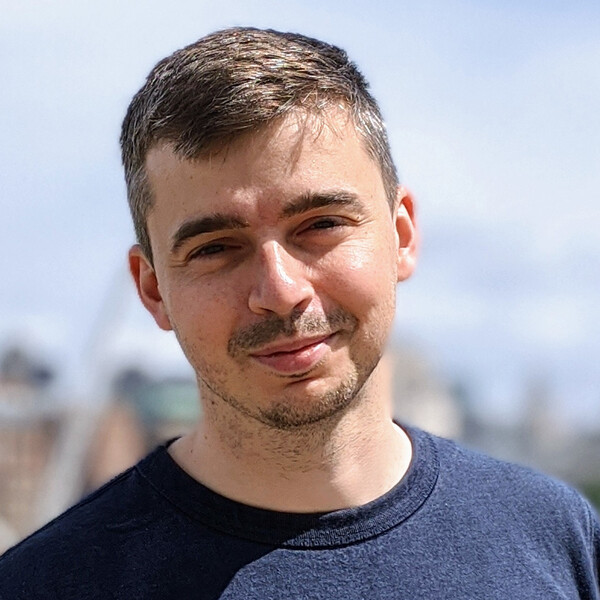
\includegraphics[width=0.06\textheight]{people/david_yallup.jpg}%
        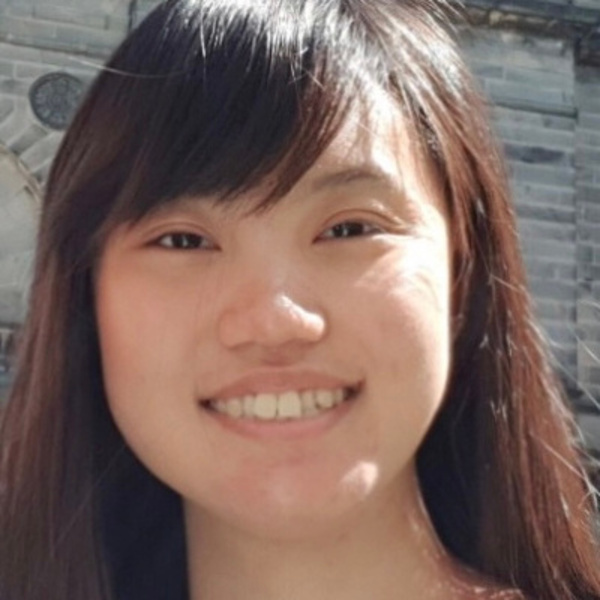
\includegraphics[width=0.06\textheight]{people/dily_ong.jpg}%
        
\includegraphics[width=0.06\textheight]{people/gemini.jpg}%
        
\includegraphics[width=0.06\textheight]{people/harry_bevins.jpg}%
        
\includegraphics[width=0.06\textheight]{people/metha_prathaban.jpg}%
        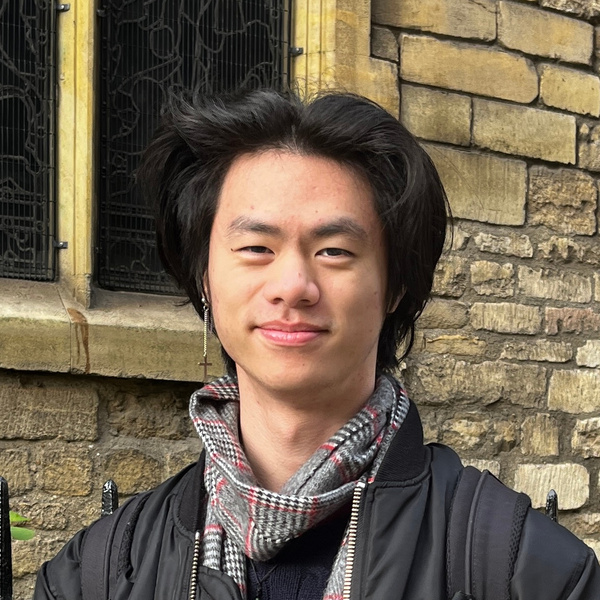
\includegraphics[width=0.06\textheight]{people/ming_yang.jpg}%
        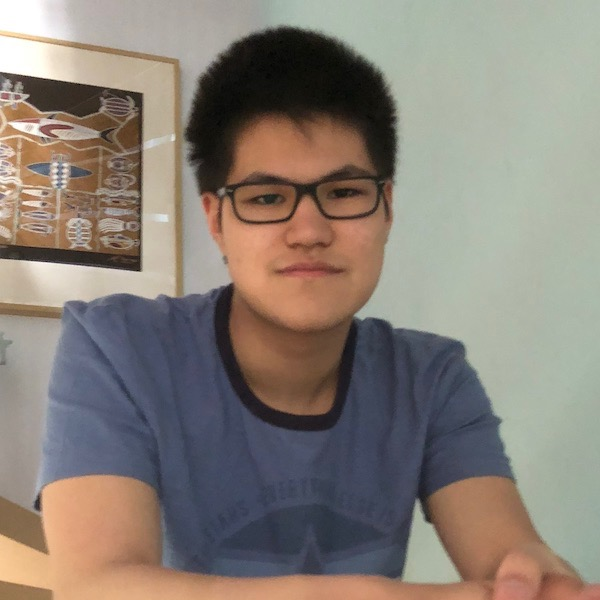
\includegraphics[width=0.06\textheight]{people/namu_kroupa.jpg}%
        
\includegraphics[width=0.06\textheight]{people/openai.jpg}%
        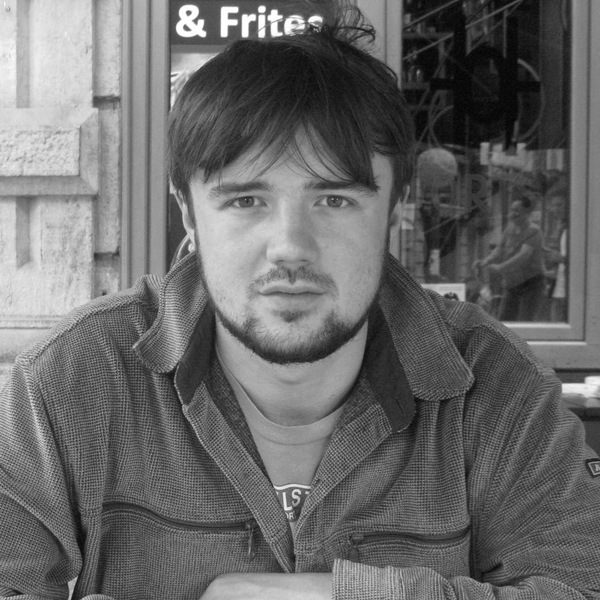
\includegraphics[width=0.06\textheight]{people/sam_leeney.jpg}%
        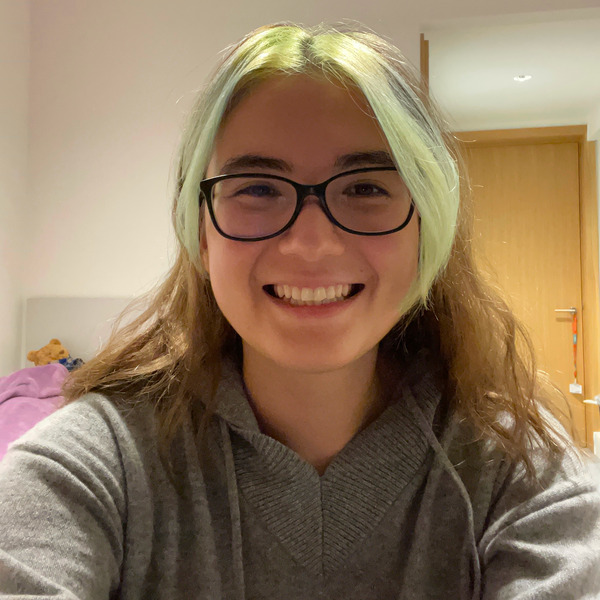
\includegraphics[width=0.06\textheight]{people/sinah_legner.jpg}%
        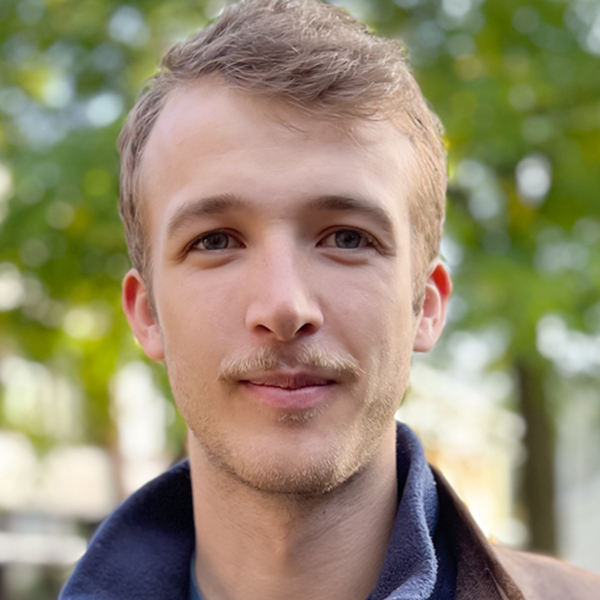
\includegraphics[width=0.06\textheight]{people/toby_lovick.jpg}%
        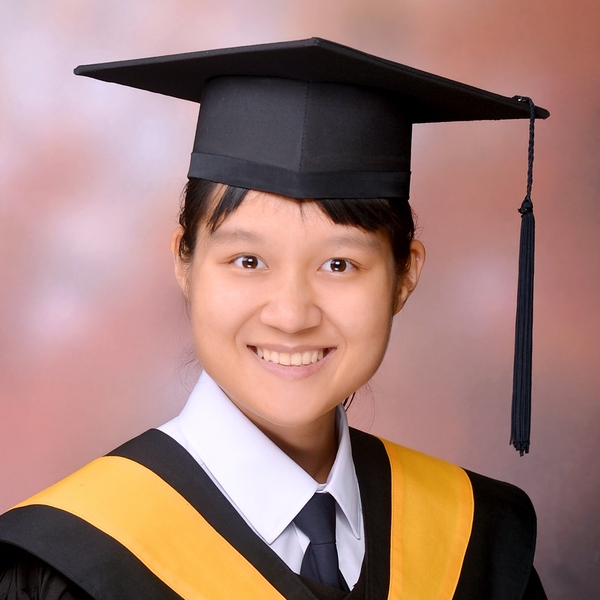
\includegraphics[width=0.06\textheight]{people/wei-ning_deng.jpg}%
        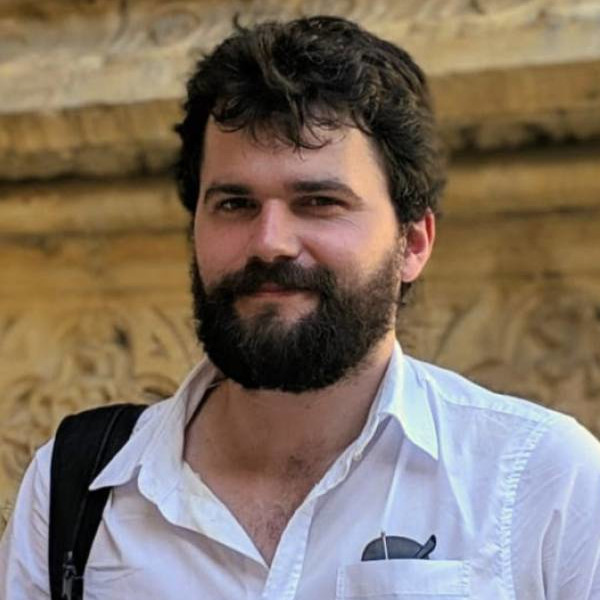
\includegraphics[width=0.06\textheight]{people/will_handley.jpg}%
        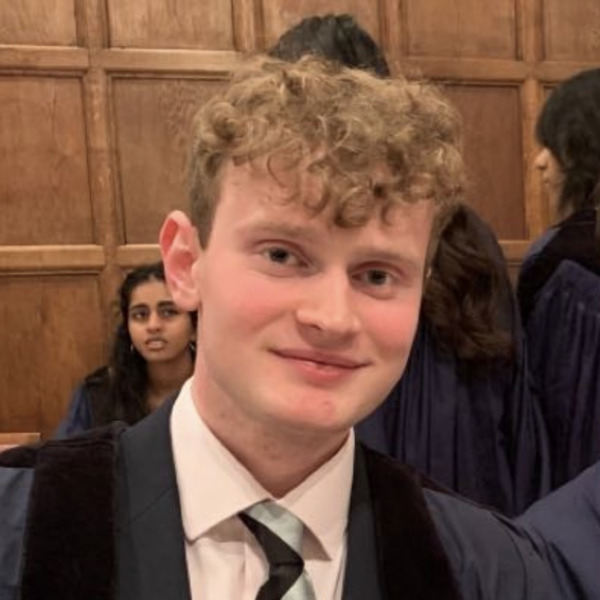
\includegraphics[width=0.06\textheight]{people/will_templeton.jpg}%
    };
\end{frame}

\end{document}
